%%%%%%%%%%%%%%%%%%%%%%%%%%%%%%%%%%%%%%%%%%%%%%%%%%%%%%%%%%%%%%%%%%%%%%
% Lớp 12 | Ứng dụng đạo hàm để khảo sát hàm số | Sự đồng biến và nghịch biến của hàm số
% Dạng 2D1?1-2: Xét tính đơn điệu dựa vào bảng biến thiên, đồ thị
% Số câu: 41  (sinh tự động bởi tach_cau.py; từ nay thầy sửa trực tiếp file này)
%%%%%%%%%%%%%%%%%%%%%%%%%%%%%%%%%%%%%%%%%%%%%%%%%%%%%%%%%%%%%%%%%%%%%%

%%%%%%%%%%%%%%%% TRẮC NGHIỆM 4 PHƯƠNG ÁN %%%%%%%%%%%%%%%%

% nguồn: Phan1_Lop_12_Dai_so_Chuong_1
\begin{ex}%[2D1N1-2]%[ma:8167dea5]
	 Hàm số $y=f(x)$ có bảng biến thiên như sau
	\begin{center}
		
\begin{tikzpicture}[scale=1,font=\footnotesize,line join=round,line cap=round,>=stealth]
			 \tkzTabInit[nocadre=true,lgt=1,espcl=3,deltacl=0.5]
				{$x$/.7,$f'(x)$/.7,$f  (x)$/2}
				 {$-\infty$,$0$,$2$,$+\infty$}
			\tkzTabLine{,-,0,+,0,-,} 
			\tkzTabVar{+/$+\infty$,-/$-1$,+/$3$,-/$-\infty$} 
		\end{tikzpicture}
	\end{center}
	Hàm số $y=f(x)$ đồng biến trên khoảng nào  dưới đây?
	 \choice
		 {$(0;+\infty)$}
		 {$(0;3)$}
		{$(-1;3)$} 
		{\True $(0;2)$} 
	 \loigiai{
		Từ  bảng biến thiên ta có $f'(x)>0$ trên khoảng $(0;2)$ do đó hàm số $y=f(x)$ đồng biến trên $(0;2)$.
	 }
\end{ex}

% nguồn: Phan1_Lop_12_Dai_so_Chuong_1
\begin{ex}%[2D1N1-2]%[ma:4c572516]
	Cho hàm số $y=f(x)$ liên tục trên  $\mathbb{R}$ và có bảng biến thiên như sau
	\begin{center}
		
\begin{tikzpicture}
			\tkzTabInit[lgt=1,espcl=3] 
				{$x$/0.7,$y'$/0.7,$y$/2} 
				{$-\infty$,$-2$,$0$,$2$,$+\infty$} 
			 \tkzTabLine{,+,0,-,0,+,0,-,}
			 \tkzTabVar{-/$-\infty$,+/ $3$/,-/$-1$,+/$3$,-/$-\infty$}
		\end{tikzpicture}
	\end{center}
	Hàm số  $y=f(x)$ nghịch biến trên khoảng nào dưới đây?
	 \choice
		{$(0;+\infty)$} 
		 {$(0;2)$}
		{$(-\infty;-2)$} 
		 {\True $(-2;0)$}
	\loigiai{ 
		Dựa vào bảng biến thiên ta có hàm số $y=f(x)$ nghịch biến  trên khoảng $(-2;0)$.
	} 
\end{ex}

% nguồn: Phan1_Lop_12_Dai_so_Chuong_1
\begin{ex}%[2D1N1-2]%[ma:66cad8d8]
	Cho hàm số $y=f(x)$ có đạo hàm  $f'(x)=2x+4$, $\forall x\in\mathbb{R}$. Hàm số đã cho nghịch biến trên khoảng nào dưới đây?
	\choice 
		 {$(2;4)$}
		 {\True $(-\infty;-2)$}
		 {$(2;+\infty)$}
		 {$(-2;+\infty)$}
	\loigiai{ 
		Ta có $f'(x)=2x+4=0\Leftrightarrow  x=-2$.\\
		Bảng  xét dấu
		\begin{center}
			
\begin{tikzpicture}
				 \tkzTabInit[lgt=1.2,espcl=3]
					 {$x$/0.7,$f'(x)$/0.7}
					{$-\infty$,$0$,$+\infty$} 
				\tkzTabLine{,-,0,+,} 
			\end{tikzpicture}
		\end{center}
		Suy ra  hàm số nghịch biến trên $(-\infty;-2)$.
	} 
\end{ex}

% nguồn: Phan1_Lop_12_Dai_so_Chuong_1
\begin{ex}%[2D1N1-2]%[ma:8df3e4fd]
	Cho hàm số $f(x)$  có bảng xét dấu của đạo hàm như sau:
	\begin{center}
		
\begin{tikzpicture}
			\tkzTabInit 
				{$x$/1,$f'(x)$/1} 
				{$-\infty$,$-3$,$0$,$2$,$+\infty$} 
			\tkzTabLine{,+,0,-,0,+,0,-,} 
		\end{tikzpicture}
	\end{center}
	Hàm số đã cho nghịch biến trên khoảng nào  dưới đây?
	 \choice
		 {\True $(-3;0)$}
		{$(0;+\infty)$} 
		 {$(0;2)$}
		{$(-\infty;-3)$} 
	\loigiai{ 
	Từ bảng xét dấu ta có $f'(x)<0$ trên khoảng $(-3;0)$. Do đó hàm số $y=f(x)$  nghịch biến trên khoảng $(-3;0)$.}
\end{ex}

% nguồn: Phan1_Lop_12_Dai_so_Chuong_1
\begin{ex}%[2D1N1-2]%[ma:39875138]
	Cho hàm số $y=f(x)$ có bảng biến thiên như sau 
	\begin{center}
		
\begin{tikzpicture}
			 \tkzTabInit[nocadre=false,lgt=1.5,espcl=2.5,deltacl=0.6]
				{$x$/0.7,$f'(x)$/0.7,$f (x)$/1.5} 
				{$-\infty$,$-1$,$0$,$1$,$+\infty$} 
			 \tkzTabLine{,+,0,-,0,+,0,-,}
			\tkzTabVar{-/$-\infty$,+/$2$,-/$1$,+/$2$,-/$-\infty$} 
		\end{tikzpicture}
	\end{center}
	 Hàm số đã cho đồng biến trên khoảng nào dưới đây?
	 \choice
		 {$(1;+\infty)$}
		{$(-1;0)$} 
		 {$(-1;1)$}
		 {\True $(0;1)$}
	\loigiai{ 
		Hàm số đã cho đồng biến trên các khoảng $(-\infty;-1)$  và $(0;1)$.
	} 
\end{ex}

% nguồn: Phan1_Lop_12_Dai_so_Chuong_1
\begin{ex}%[2D1N1-2]%[ma:e42229d3]
	 Cho hàm số $f(x)=ax^3+bx^2+cx+d$ ($a$, $b$, $c$, $d\in \mathbb{R}$, $a\neq 0$) có bảng xét dấu của đạo hàm dưới đây.
	\begin{center}
		
\begin{tikzpicture}[scale=1,font=\footnotesize,line join=round,line cap=round,>=stealth]
			 \tkzTabInit[nocadre=True,lgt=1,espcl=3,deltacl=0.5]
				 {$x$/.7,$f'(x)$/.7}
				 {$-\infty$,$5$,$6$,$+\infty$}
			\tkzTabLine{,-,0,+,0,-,} 
		\end{tikzpicture}
	\end{center}
	 Hàm số đã cho đồng biến trên khoảng
	 \choice
		{$(-\infty;5)$} 
		{\True $(5;6)$} 
		{$(5;+\infty)$} 
		{$(6;+\infty)$} 
	 \loigiai{
		Từ bảng biến thiên suy ra hàm số đồng biến  trên khoảng $(5;6)$.
	 }
\end{ex}

% nguồn: Phan1_Lop_12_Dai_so_Chuong_1
\begin{ex}%[2D1N1-2]%[ma:88ca446b]
	Cho hàm  số $y=f(x)$ liên tục trên $\mathbb{R}$ và có bảng biến thiên như sau
	\begin{center}
		
\begin{tikzpicture}
			 \tkzTabInit[lgt=1.2,espcl=2]
				 {$x$ /.7,$f (x)$ /2}
				{$-\infty$,$-1$,$1$,$+\infty$} 
			 \tkzTabVar{-/$-\infty$,+/$3$,-/$0$,+/$+\infty$}
		\end{tikzpicture}
	\end{center}
	Hàm số  đã cho nghịch biến trên khoảng
	 \choice
		 {$\left(-2;1\right)$}
		 {\True $\left(0;1\right)$}
		 {$\left(0;3\right)$}
		{$\left(1;+\infty\right)$} 
	 \loigiai{
		Dựa vào bảng biến thiên ta thấy hàm  số nghịch biến trên $\left(-1;1\right)$ và $\left(0;1\right)\subset\left(-1;1\right)$.
	 }
\end{ex}

% nguồn: Phan1_Lop_12_Dai_so_Chuong_1
\begin{ex}%[2D1N1-2]%[ma:7b064781]
	Cho hàm số $y=f(x)$ có đạo hàm  trên $\mathbb{R}$ và có bảng xét dấu của đạo hàm như sau:
	\begin{center}
		\resizebox{0.8\linewidth}{!}{
\begin{tikzpicture}
		\tkzTabInit[nocadre,espcl=2.5] 
			{$x$/0.8,$f'(x)$/0.8} 
			{$-\infty$,$2$,$5$,$8$,$+\infty$} 
		\tkzTabLine{,-,0,+,0,-,0,+,} 
	\end{tikzpicture}
		 }
	\end{center}
	Hàm số đã cho  đồng biến trên khoảng
	 \choice
		 {$(-\infty;2)$}
		 {$(5;8)$}
		{\True $(3;4)$} 
		{$(5;+\infty)$} 
	\loigiai{ 
		Dựa vào bảng  xét dấu của $f'(x)$, ta có hàm số đồng biến trên các khoảng $(2;5)$ và $(8;+\infty)$ nên hàm số đồng biến trên khoảng $(3;4)$.
	} 
\end{ex}

% nguồn: Phan1_Lop_12_Dai_so_Chuong_1
\begin{ex}%[2D1N1-2]%[ma:2623c99f]
	Cho hàm số $y=f(x)$  có bảng biến thiên như sau:
	\begin{center}
		
\begin{tikzpicture}
			 \tkzTabInit[nocadre,lgt=1.2,espcl=2.5,deltacl=0.6]
				 {$x$/0.8,$y'$/0.8,$y$/2}
				{$-\infty$,$0$,$1$,$+\infty$} 
			\tkzTabLine{,+,0,-,0,+,} 
			 \tkzTabVar{-/$-\infty$,+/$0$,-/$-1$,+/$+\infty$}
		\end{tikzpicture}
	\end{center}
	Hàm số $y=f(x)$ đồng biến trên khoảng 
	 \choice
		{$(-1;+\infty)$} 
		 {$(-\infty;1)$}
		 {$(0;1)$}
		{\True  $(-3;-2)$}
	\loigiai{ 
		Dựa vào bảng biến thiên của hàm số $y=f(x)$, ta có hàm số  đồng biến trên các khoảng $(-\infty;0)$ và $(1;+\infty)$ nên hàm số đồng biến trên khoảng $(-3;-2)$.
	 }
\end{ex}

% nguồn: Phan1_Lop_12_Dai_so_Chuong_1
\begin{ex}%[2D1N1-2]%[ma:d4f22c65]
	Cho hàm số $y=f(x)$ có bảng xét dấu đạo hàm  như sau
	\begin{center}
		
\begin{tikzpicture}[font=\footnotesize,>=stealth]
		\tikzset{double style/.append style={double distance=1.5pt}}
		 \tkzTabInit[nocadre=false,lgt=1.2,espcl=2.5,deltacl=0.6]
			{$x$ /0.7,$y'$  /0.6}
			{$-\infty$,$-2$,$0$,$2$,$+\infty$} 
		 \tkzTabLine{,+,$0$,-,d,-,$0$,+,}
	\end{tikzpicture}
	\end{center}
	Mệnh đề nào dưới đây  đúng?
	 \choice
		{Hàm số nghịch biến trên khoảng  $(-\infty;-2)$}
		{Hàm số  đồng biến trên khoảng $(-2;0)$}
		{Hàm số đồng biến trên  khoảng $(-\infty;0)$}
		{\True Hàm số nghịch  biến trên khoảng $(0;2)$}
	\loigiai{ 
		Dựa vào bảng xét dấu ta thấy hàm số  nghịch biến trên khoảng $(0;2)$.
	} 
\end{ex}

% nguồn: Phan1_Lop_12_Dai_so_Chuong_1
\begin{ex}%[2D1N1-2]%[ma:8678744f]
	Cho hàm số $f(x)$  có bảng xét dấu của $f'(x)$ như sau:
	\begin{center}
		
\begin{tikzpicture}[scale=0.9,>=stealth]
			 \tkzTabInit[nocadre=false,lgt=2,espcl=2.7,deltacl=0.6]
				 {$x$/0.8,$f'(x)$/0.8}
				 {$-\infty$,$-3$,$0$,$2$,$4$,$+\infty$}
			\tkzTabLine{,-,$0$,+,$0$,-,d,-,$0$,+,} 
		\end{tikzpicture}
	\end{center}
	Hàm số đã  cho nghịch biến trên khoảng nào dưới đây?
	 \choice
		{$(-\infty;  0)$}
		 {\True $(0; 2)$}
		 {$(4;+\infty)$}
		{$(0;  4)$}
	 \loigiai{
		Hàm số đã cho nghịch biến trên khoảng $(0;  2)$.
	 }
\end{ex}

% nguồn: Phan1_Lop_12_Dai_so_Chuong_1
\begin{ex}%[2D1N1-2]%[ma:29d08c8a]
	Cho hàm số $y=\dfrac{ax^2+bx+c}{mx+n}~(a, b, c, m, n \in \mathbb{R}, am \neq 0)$ có bảng xét dấu  của đạo hàm như sau:
	\begin{center}
		\resizebox{0.8\linewidth}{!}{
\begin{tikzpicture}
		 \tkzTabInit[nocadre,espcl=2.5]
			{$x$/0.8,$f'(x)$/0.8} 
			{$-\infty$,$4$,$7$,$10$,$+\infty$} 
		\tkzTabLine{,+,0,-,d,+,0,-,} 
	\end{tikzpicture}
		 }
	\end{center}
	Hàm số đã cho nghịch biến trên khoảng 
	 \choice
		{\True  $(11;12)$}
		{$(7;10)$} 
		{$(-\infty;7)$} 
		{$(4;+\infty)$} 
	 \loigiai{
		Dựa vào bảng xét  dấu của $f'(x)$, ta có hàm số nghịch biến trên các khoảng $(4;7)$ và $(10;+\infty)$ nên hàm số nghịch biến trên khoảng $(11;12)$.
	} 
\end{ex}

% nguồn: Phan1_Lop_12_Dai_so_Chuong_1
\begin{ex}%[2D1N1-2]%[ma:17f25550]
	\immini{ 
	Cho hàm số $y=f(x)$ có đạo hàm trên $\mathbb{R}$ và hàm số $y=f'(x)$ là hàm số bậc ba có đồ thị là đường cong trong hình vẽ. Hàm số $y=f(x)$ nghịch biến  trên
	\choice 
		{\True $(-\infty;1)$} 
		 {$(-2;0)$}
		 {$(1;+\infty)$}
		 {$(-1;+\infty)$}
		}{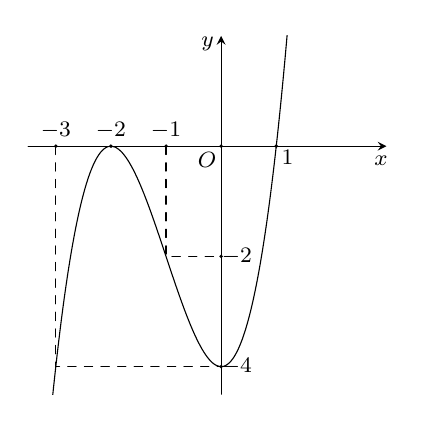
\begin{tikzpicture}[scale=0.7,font=\footnotesize,line join=round,
			line cap=round,>=stealth] 
		\def \xmin{-3.5} 
		 \def \xmax{3}
		\def  \ymin{-4.5}
		 \def \ymax{2}
		 \draw[->] (\xmin,0)--(\xmax,0) node[shift=(-110:0.2)] {$x$};
		\draw[->] (0,\ymin)--(0,\ymax) node[shift=(-150:0.2)] {$y$}; 
		\fill (0,0)  circle (1pt) node[shift=(-135:0.25)]{$O$}
			(-3,0) circle  (1pt) node[shift=(90:0.2)]{$-3$}
			(-2,0) circle  (1pt) node[shift=(90:0.2)]{$-2$}
			 (-1,0) circle (1pt) node[shift=(90:0.2)]{$-1$}
			(1,0) circle (1pt)  node[shift=(-45:0.2)]{$1$}
			(0,-4)  circle (1pt) node[shift=(0:0.2)]{$-4$}
			(0,-2) circle  (1pt) node[shift=(0:0.2)]{$-2$};
		\draw[dashed] (-3,0)|-(0,-4) 
			(-1,0)|-(0,-2); 
		\clip  (\xmin,\ymin) rectangle (\xmax,\ymax);
		\draw[smooth,samples=100,domain=\xmin:\xmax]  plot (\x,{(\x)^3+3*(\x)^2-4});
	\end{tikzpicture}
		 }
	\loigiai{Dựa vào đồ thị, ta thấy $f'(x) <  0$, $\forall x < 1$. Do đó hàm số nghịch biến trên khoảng $(-\infty;1)$.}
\end{ex}

% nguồn: Phan1_Lop_12_Dai_so_Chuong_1
\begin{ex}%[2D1N1-2]%[ma:7c47a278]
	Cho hàm số $y=f(x)$ liên tục $\mathbb R$ và có bảng biến thiên như sau.  Hỏi hàm số đồng biến trên khoảng nào?
	\begin{center}
		\begin{tikzpicture}
			 \tkzTabInit[nocadre=true,lgt=1.2,espcl=1.8,deltacl=0.4]
				{$x$/0.75,$f'(x)$/0.75,$f  (x)$/2}{$-\infty$,$-1$,$0$,$1$,$+\infty$}
			\tkzTabLine{,+,0,-,0,+,0,-,} 
			 \path
				 (N13) node[shift={(0,0)}](A){$-\infty$}
				 (N22) node[shift={(0,-0.3)}](B){$-1$}
				(N33)  node[shift={(0,0.4)}](C){$-2$}
				(N42) node[shift={(0,-0.3)}](D){$-1$} 
				 (N53) node[shift={(0,0)}](E){$-\infty$};
			 \foreach\X/\Y in{A/B,B/C,C/D,D/E}\draw[-stealth](\X)--(\Y);
		\end{tikzpicture}
	\end{center}
	\choice 
		 {\True $\left( 0;1 \right)$}
		{$\left(  -1;0 \right)$}
		{$\left( -\infty;1 \right)$} {$\left( 1;+\infty \right)$} 
	\loigiai{Dựa vào bảng biến thiên ta có hàm số  đồng biến trên $\left( 0;1 \right)$.}
\end{ex}

% nguồn: Phan1_Lop_12_Dai_so_Chuong_1
\begin{ex}%[2D1N1-2]%[ma:40063c84]
	Cho hàm số $y=f(x)$ có bảng xét dấu của đạo hàm $f'(x)$ trên $\mathbb{R}$  như hình vẽ
	\begin{center}
		
\begin{tikzpicture}
			\tkzTabInit 
				{$x$/1,$f'(x)$/1} 
				{$-\infty$,$-1$,$+\infty$} 
			\tkzTabLine{,-,0,+,} 
		\end{tikzpicture}
	\end{center}
	Hàm số $y=f(x)$ đồng biến  trên khoảng
	\choice 
		{$(-\infty;-1)$} 
		 {$\mathbb{R}$}
		 {\True $(-1;+\infty)$}
		 {$(-2;+\infty)$}
	\loigiai{ 
	Từ bảng xét dấu ta có $f'(x)>0$  trên khoảng $(-1;+\infty)$. Do đó hàm số $y=f(x)$ đồng biến trên khoảng $(-1;+\infty)$.}
\end{ex}

% nguồn: Phan1_Lop_12_Dai_so_Chuong_1
\begin{ex}%[2D1N1-2]%[ma:0ecf7772]
	\immini{Cho hàm số $ y=f(x)=ax^3+bx^2+cx+d$ có  đồ thị như hình vẽ bên. Hàm số $ y=f(x)$ đồng biến trên khoảng nào?
	\choice 
		 {$(-1;1)$}
		{$(-\infty;-1)$} 
		{$(2;+\infty)$} 
		{\True $(0;1)$}}{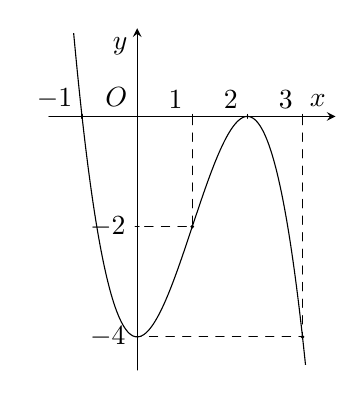
\begin{tikzpicture}[line join=round,line cap=round,>=stealth,scale=0.7]
		\tikzset{ethicknode/.style={scale=0.7}} 
		\draw[->] (-1.6,0)--(3.6,0)  node[above left] {$x$};
		\draw[->] (0,-4.6)--(0,1.6) node[below left]  {$y$};
		\draw (0,0) node [above left] {$O$}; 
		 \foreach \x/\nx in {-1/-1,1/1,2/2,3/3}
		\draw[thin] (\x,1pt)--(\x,-1pt) node  [above left] {$\nx$};
		 \foreach \y/\ny in {-2/-2,-4/-4}
		\draw[thin] (1pt,\y)--(-1pt,\y) node  [left] {$\ny$};
		\draw[dashed,thin](1,0)--(1,-2)--(0,-2); 
		 \draw[dashed,thin](3,0)--(3,-4)--(0,-4);
		\begin{scope}
			\clip (-1.5,-4.5) rectangle  (3.5,1.5);
			\draw[samples=200,domain=-1.5:4,smooth,variable=\x] plot  (\x,{-1*((\x)^3)+3*((\x)^2)+0*(\x)+-4});
		\end{scope}
		\fill (1,-2)  circle (1pt)
			(3,-4) circle  (1pt);
	\end{tikzpicture}
		} 
	 \loigiai{
	Quan sát đồ thị, ta thấy  hàm số $ y=f(x)$ đồng biến trên khoảng $(0;1)$.}
\end{ex}

% nguồn: Phan1_Lop_12_Dai_so_Chuong_1
\begin{ex}%[2D1N1-2]%[ma:0d789e15]
	Cho hàm số $y=f(x)$ có bảng xét  dấu đạo hàm như sau
	\begin{center}
		
\begin{tikzpicture}[scale=.75,transform shape]
			 \tkzTabInit[nocadre=false,lgt=1.2,espcl=2.5,deltacl=0.6]{$x$ /1,$f'(x)$ /1}
				{$-\infty$,$1$,$2$,$3$,$4$,$+\infty$} 
			 \tkzTabLine{,-,0,+,0,+,0,-,0,+,}
		\end{tikzpicture}
	\end{center}
	Hàm số đã cho đồng biến trên khoảng nào dưới  đây?
	\choice 
		{\True $\left(1;3\right)$} 
		 {$\left(3;4\right)$}
		 {$\left(2;4\right)$}
		{$\left(-\infty;-1\right)$} 
	\loigiai{Từ bảng xét dấu  ta có $f'(x)>0$ trên khoảng $\left(1;3\right)$. \\
		Vậy hàm số  đồng biến trên khoảng $\left(1;3\right)$.
	} 
\end{ex}

% nguồn: Phan1_Lop_12_Dai_so_Chuong_1
\begin{ex}%[2D1N1-2]%[ma:c1289397]
	\immini{Cho hàm số  $y=f(x)$ có đồ thị đạo hàm $y=f'(x)$ như hình vẽ bên. Hàm số $y=f(x)$ đồng biến trên khoảng
	\choice 
		 {$(-2;0)$}
		{$(0;2)$} 
		 {\True $(1;3)$}
		{$(3;4)$} 
		}{\resizebox{!}{5cm}{\begin{tikzpicture}[scale=0.75,line join=round,line cap=round,>=stealth]
		 \draw[step=1,cyan!50] (-2.5,-3.8) grid (4.25,3.8);
		\draw[->] (-2.5,0)--(4.5,0)  node[below] {$x$};
		\draw[->] (0,-4)--(0,4) node[left]  {$y$};
		\draw (0,0) node [below left] {$O$}; 
		\foreach \x in {-2,2,4}\draw (\x,0.1)--(\x,-0.1) node [below] {$\x$}; 
		\foreach \y in  {-1,1,2,3}\draw (0.1,\y)--(-0.1,\y) node [left] {$\y$};
		\draw  (-1,0.1)--(-1,-0.1);
		\fill ($(45+180:4.5mm)+(-1,0)$)  node {$-1$};
		\draw (1,0.1)--(1,-0.1); 
		 \fill ($(-45:3.5mm)+(1,0)$) node {$1$};
		\draw  (3,0.1)--(3,-0.1);
		\fill ($(-45:3.5mm)+(3,0)$)  node {$3$};
		\draw (0.1,-2)--(-0.1,-2); 
		\fill ($(180:3.8mm)+(0,-2)$) node  {$-2$};
		\draw  (0.1,-3)--(-0.1,-3);
		\fill  ($(45+180:4.5mm)+(0,-3)$) node {$-3$};
		 \draw[smooth,samples=100] plot[domain=-1.37:3.37] (\x,{-(\x)^3+3*(\x)^2+(\x)-3});
	\end{tikzpicture}
	 }}
	\loigiai{ 
		Dựa vào đồ thị của hàm số $y=f'(x)$, ta có hàm số đồng  biến trên khoảng $(1;3)$.
	 }
\end{ex}

% nguồn: Phan1_Lop_12_Dai_so_Chuong_1
\begin{ex}%[2D1N1-2]%[ma:5aa2fc50]
	Cho hàm số  có bảng biến thiên như sau
	\begin{center}
		
\begin{tikzpicture}
			\tkzTabInit[nocadre=false,lgt=1,espcl=2] 
				{$x$ /1,$y'$  /0.7,$y$ /2.2}
				 {$-\infty$,$\dfrac{-4}{3}$,$\dfrac{1}{2}$,$+\infty$}
			\tkzTabLine{,+,0,-,0,+,} 
			\tkzTabVar{-/$-\infty$,+/ $\dfrac{218}{27}$,-/ $\dfrac{-17}{4}$ /,+/$+\infty$  /}
		\end{tikzpicture}
	\end{center}
	Khẳng định  nào sau đây là \textbf{đúng}?
	\choice 
		 {Hàm số nghịch biến trên khoảng $\left(-\infty;-\dfrac{4}{3}\right)$}
		{Hàm số đồng biến trên  khoảng $\left(-\dfrac{4}{3};\dfrac{1}{2}\right)$}
		{Hàm số nghịch  biến trên khoảng $\left(\dfrac{7}{2};+\infty\right)$}
		{\True Hàm số đồng biến  trên khoảng $\left(-\infty;-\dfrac{7}{3}\right)$}
	 \loigiai{
		Dựa vào  bảng biến thiên ta thấy, hàm số đồng biến trên mỗi khoảng $\left(-\infty;-\dfrac{4}{3}\right)$ và $\left(\dfrac{1}{2};+\infty\right)$.\\
		Hàm số  nghịch biến trên $\left(-\dfrac{4}{3};\dfrac{1}{2}\right)$.
	} 
\end{ex}

% nguồn: Phan1_Lop_12_Dai_so_Chuong_1
\begin{ex}%[2D1N1-2]%[ma:7dda853b]
	 \immini{
	Cho hàm số $y=f(x)$ có đồ thị là đường cong như hình bên. Hàm số  đã cho nghịch biến trên khoảng nào dưới đây?
	\choice 
		{$(-1;1)$} 
		{\True $(1;+\infty)$} 
		 {$(0;1)$}
		 {$(-1;+\infty)$}
		 }{
		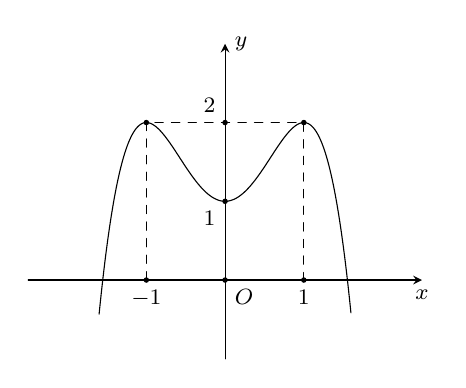
\begin{tikzpicture} [scale=1,font=\footnotesize,line join=round,line cap=round,>=stealth]
			 \draw[->] (-2.5,0)--(0,0) node[below right]{$O$}--(2.5,0) node[below]{$x$};
			\draw[->]  (0,-1)--(0,3) node[right]{$y$};
			\draw[samples=300,domain=-1.6:1.6,smooth]  plot (\x,{-(\x)^4 + 2*(\x)^2+1});
			\foreach \i in {(0,0),(-1,0),(-1,2),(1,0),(1,2),(0,1),(0,2)} \fill  \i circle (1pt);
			\draw (0,1) node[below left]{$1$}; 
			\draw[dashed] (-1,0) node[below]{$-1$}--(-1,2)--(0,2)  node[above left]{$2$}--(1,2)--(1,0) node[below]{$1$};
		\end{tikzpicture}
		 }
	\loigiai{ 
		Dựa vào đồ thị  ta thấy hàm số $y=f(x)$ nghịch biến trên khoảng $(-1;0)$ và $(1;+\infty)$.
	 }
\end{ex}

% nguồn: Phan1_Lop_12_Dai_so_Chuong_1
\begin{ex}%[2D1N1-2]%[ma:c2fe05fb]
	Cho hàm số $f(x)$ có bảng biến thiên như  sau:
	\begin{center}
		
\begin{tikzpicture}
			 \tkzTabInit[espcl=2.5,lgt=1.5]
				 {$x$/0.7,$y'$/0.7,$y$/2.1}
				{$-\infty$,$-1$,$3$,$+\infty$} 
			\tkzTabLine{,+,0,-,0,+,} 
			 \tkzTabVar{-/$-\infty$,+/$1$,-/$-3$,+/$+\infty$}
		\end{tikzpicture}
	\end{center}
	 Hàm số đã cho đồng biến trên khoảng nào sau đây?
	\choice 
		 {$(-\infty;1)$}
		{\True  $(3;+\infty)$}
		{$(-1;3)$} 
		{$(-3;+\infty)$} 
	\loigiai{ 
		Từ bảng biến thiên ta thấy hàm số đồng biến trên  các khoảng $(-\infty;-1)$ và $(3;+\infty)$.
	} 
\end{ex}

% nguồn: Phan1_Lop_12_Dai_so_Chuong_1
\begin{ex}%[2D1N1-2]%[ma:082e92f7]
	Cho hàm số $f(x)$ có bảng  xét dấu của đạo hàm như sau:
	\begin{center}
		
\begin{tikzpicture}
			 \tkzTabInit[nocadre=true,lgt=1.2,espcl=3,deltacl=0.5]
				{$x$/0.7,$f'(x)$/0.7} 
				{$-\infty$,$-3$,$2$,$+\infty$} 
			\tkzTabLine{,+,0,+,0,-,} 
		\end{tikzpicture}
	\end{center}
	Hàm số đã cho nghịch biến  trên khoảng nào dưới đây?
	 \choice
		{\True $(2;+\infty)$} 
		 {$(-\infty;-2)$}
		{$(-2;+\infty)$} 
		 {$(-2;1)$}
	\loigiai{ 
		Từ bảng xét dấu đạo hàm suy ra hàm số nghịch biến trên khoảng  $(2;+\infty)$.
	} 
\end{ex}

% nguồn: Phan1_Lop_12_Dai_so_Chuong_1
\begin{ex}%[2D1N1-2]%[ma:8b06e4db]
	Cho  hàm số $y=f(x)$ liên tục trên $\mathbb{R}$ và có bảng biến thiên như sau.
	\begin{center}
		\resizebox{0.7\linewidth}{!}{
\begin{tikzpicture}
		 \tkzTabInit[nocadre=true,lgt=1.2,espcl=3,deltacl=0.5]
			{$x$/0.7,$f'(x)$/0.7,$f (x)$/2} 
			{$-\infty$,$0$,$2$,$+\infty$} 
		 \tkzTabLine{,+,0,-,0,+,}
		 \tkzTabVar{-/$-\infty$,+/$4$,-/$0$,+/$+\infty$}
	\end{tikzpicture}
		 }
	\end{center}
	Hàm số đã cho nghịch  biến trên khoảng nào dưới đây?
	\choice 
		{\True  $(0;2)$}
		{$(0;+\infty)$} 
		 {$(-\infty; 0)$}
		{$(-\infty; 2)$} 
	 \loigiai{
		Dựa vào bảng biến thiên  ta thấy hàm số nghịch biến trên khoảng $(0;2)$.
	} 
\end{ex}

% nguồn: Phan1_Lop_12_Dai_so_Chuong_1
\begin{ex}%[2D1N1-2]%[ma:3a4c3759]
	\immini{Cho hàm số có đồ thị như hình bên. Khẳng định nào sau đây  là \textbf{đúng}?
	\choice 
		{Hàm số  nghịch biến trên khoảng $(-\infty;1)$}
		 {Hàm số nghịch biến trên khoảng $(-\infty;0)$}
		{Hàm số nghịch biến trên khoảng  $\left(\dfrac{7}{3};+\infty\right)$}
		 {\True Hàm số đồng biến trên khoảng $(-\infty;1)$}
		 }{
		\begin{tikzpicture}[line cap=round,>=stealth,scale=0.4]
			\tikzset{ethicknode/.style={scale=0.5}} 
			\draw[->] (-3.333,0)--(6.667,0) node[below left] {$x$}; 
			 \draw[->] (0,-3.593)--(0,10.407) node[below left] {$y$};
			\draw  (0,0) node [below left] {$O$};
			\draw[dashed](1,0)  node[below] {$1$}--(1,4)
				(2.333,0) node[below]  {$\dfrac{7}{3}$}--(2.333,2.815);
			\begin{scope}
				 \clip (-3.333,-3.493) rectangle (6.667,10.307);
				\draw[samples=100,domain=-3.233:6.567,smooth,variable=\x] plot  (\x,{1*((\x)^3)-5*((\x)^2)+7*(\x)+1});
			\end{scope}
		\end{tikzpicture}
		} 
	\loigiai{ 
		Dựa vào đồ thị ta thấy, hàm số đồng biến trên  mỗi khoảng $(-\infty;1)$ và $\left(\dfrac{7}{3};+\infty\right)$.\\
		 Hàm số nghịch biến trên $\left(1;\dfrac{7}{3}\right)$.
	} 
\end{ex}

% nguồn: Phan1_Lop_12_Dai_so_Chuong_1
\begin{ex}%[2D1N1-2]%[ma:2302c99f]
	Cho hàm số $y=f(x)$ có  bảng xét dấu đạo hàm như sau:\\
	\begin{center}
		\resizebox{0.7\linewidth}{!}{
\begin{tikzpicture}
		\tkzTabInit[nocadre,espcl=2.5,lgt=1.5] 
			{$x$/0.7,$f'(x)$/0.7} 
			{$-\infty$,$-2$,$0$,$1$,$+\infty$} 
		 \tkzTabLine{,-,d,+,0,+,d,-,}
	\end{tikzpicture}
		 }
	\end{center}
	Hàm số đã  cho đồng biến trên khoảng nào sau đây?
	 \choice
		 {$\left(-2;2\right)$}
		 {$\left(-2;+\infty\right)$}
		{$\left(-\infty;0\right)$} 
		{\True $\left(-2;1\right)$} 
	 \loigiai{
	Hàm số đồng biến trên $\left(-2;1\right)$.} 
\end{ex}

% nguồn: Phan1_Lop_12_Dai_so_Chuong_1
\begin{ex}%[2D1N1-2]%[ma:941c5953]
	 Cho hàm số $y=f(x)$ xác định với mọi $x\ne-6$ có bảng biến thiên như hình vẽ dưới đây.
	\begin{center}
		
\begin{tikzpicture}[>=stealth]
			 \tkzTabInit[nocadre=false,lgt=1,espcl=2,deltacl=0.5]{$x$/.7,$y'$/.7,$y$/2}
				 {$-\infty$,$-7$,$-6$,$0$,$+\infty$}
			\tkzTabLine{,-,$0$,+,d,+,$0$,-,} 
			 \tkzTabVar{+/$+\infty$,-/$-12$,+D-/$+\infty$/$-\infty$,+/$-15$,-/$-\infty$}
		\end{tikzpicture}
	\end{center}
	Hàm số đồng biến  trên khoảng nào trong các khoảng sau?
	\choice 
		{$(-6;+\infty)$} 
		 {$(0;+\infty)$}
		 {$(-10;1)$}
		 {\True$(-7;-6)$}
	 \loigiai{
		Dựa vào bảng biến thiên, ta thấy với mọi $x\in(-7;-6)$,  $f'(x)>0$.\\
		Nên hàm số  đồng biến trên khoảng $(-7;-6)$.
	} 
\end{ex}

% nguồn: Phan1_Lop_12_Dai_so_Chuong_1
\begin{ex}%[2D1N1-2]%[ma:f41cab9e]
	Cho hàm số $y=f(x)$  có bảng biến thiên như sau:
	\begin{center}
		\resizebox{0.8\linewidth}{!}{
\begin{tikzpicture}
		\tkzTabInit[nocadre,espcl=2.5] 
			{$x$/0.8,$y'$/0.8,$y$/2} 
			 {$-\infty$,$-1$,$0$,$1$,$+\infty$}
		\tkzTabLine{,+,0,-,d,-,0,+,} 
		 \tkzTabVar{-/$-\infty$,+/$-2$,-D+/$-\infty$/$+\infty$,-/$-2$,+/$+\infty$}
	\end{tikzpicture}
		 }
	\end{center}
	Hàm số nghịch  biến trên khoảng
	\choice 
		{$(-1;1)$} 
		 {$(-\infty;-2)$}
		{\True  $(0;1)$}
		{$(2;+\infty)$} 
	\loigiai{ 
		Dựa vào bảng biến thiên của hàm số $y=f(x)$,  ta có hàm số nghịch biến trên các khoảng $(-1;0)$ và $(0;1)$ nên hàm số nghịch biến trên khoảng $(0;1)$.
	} 
\end{ex}

% nguồn: Phan1_Lop_12_Dai_so_Chuong_1
\begin{ex}%[2D1N1-2]%[ma:b027bd38]
	Cho hàm số $ f(x)$ có bảng xét dấu của đạo  hàm như sau
	\begin{center}
		
\begin{tikzpicture}[font=\footnotesize,>=stealth]
		\tikzset{double style/.append style={double distance=1.5pt}}
		\tkzTabInit[nocadre=false,lgt=1.2,espcl=2.5,deltacl=0.6] 
			{$x$ /0.7,$f'(x)$  /0.6}
			 {$-\infty$,$-3$,$0$,$2$,$+\infty$}
		\tkzTabLine{,+,$0$,-,$0$,+,$0$,-,} 
	\end{tikzpicture}
	\end{center}
	Hàm số đã cho nghịch biến trên khoảng  nào dưới đây?
	 \choice
		{\True  $(-3;0)$}
		 {$(0;+\infty)$}
		{$(0;2)$} 
		{$(-\infty;-3)$} 
	 \loigiai{
		Ta  có bảng biến thiên
		\begin{center}
			
\begin{tikzpicture}[font=\footnotesize,>=stealth]
			\tikzset{double style/.append style={double distance=1.5pt}}
			 \tkzTabInit[nocadre=false,lgt=1.2,espcl=2.5,deltacl=0.6]
				{$x$  /0.7,$f'(x)$ /0.6,$f (x)$/2}
				{$-\infty$,$-3$,$0$,$2$,$+\infty$} 
			\tkzTabLine{,+,$0$,-,$0$,+,$0$,-,} 
			 \tkzTabVar{-/,+/,-/,+/,-/}
		\end{tikzpicture}
		\end{center}
		Dựa vào bảng biến thiên suy ra hàm  số nghịch biến trên $(-3;0)$.
	} 
\end{ex}

% nguồn: Phan1_Lop_12_Dai_so_Chuong_1
\begin{ex}%[2D1H1-2]%[ma:65c5f0a0]
	\immini{Cho đồ thị của hàm $y=f(x)$ có đồ thị như  hình vẽ bên dưới. Hàm số đã cho đồng biến trên khoảng nào dưới đây?
	\choice 
		{$\left( {1;\, + \infty } \right)$} 
		{\True $\left( -\infty;\,0 \right)$} 
		{$\left( 2;\,3  \right)$}
		{$\left( 1;\,3 \right)$}}{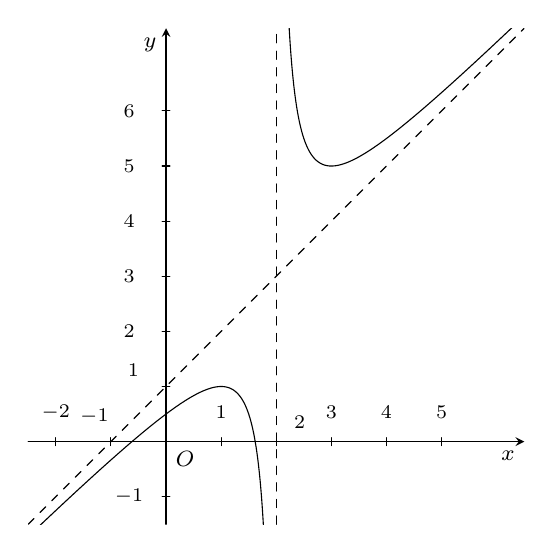
\begin{tikzpicture}[scale=0.7,font=\footnotesize,line join=round,line cap=round,>=stealth]
		\def \a{1} 
		\def \b{-1} 
		\def \c{-1} 
		\def \u{1} 
		\def  \v{-2}
		 \def \f{((\a)*(\x)^2+(\b)*(\x)+(\c))/((\u)*(\x)+(\v))}
		 \def \tcx{(\x)+1}
		\def  \xo{-{\v/\u}}
		\def \yo{\xo+1} 
		\def  \kx{4.5}
		\draw[->] (\xo-\kx,0)--(\xo+\kx,0)  node[below left] {$x$};
		\draw[->] (0,\yo-\kx)--(0,\yo+\kx) node[below left]  {$y$};
		 \draw (0,0) node [below right] {$O$};
		\foreach \x/\g in {-2/90,-1/120,1/90,2/45,3/90,4/90,5/90} 
		\draw[thin]  (\x,2pt)--(\x,-2pt) + (\g:6mm) node {\scriptsize $\x$};
		 \foreach \y/\g in {-1/180,1/150,2/180,3/180,4/180,5/180,6/180}
		\draw[thin] (2pt,\y)--(-2pt,\y)  + (\g:6mm) node {\scriptsize $\y$};
		\begin{scope}
			 \clip (\xo-\kx,\yo-\kx) rectangle (\xo+\kx,\yo+\kx);
			 \draw[smooth,samples=200,domain=\xo-\kx:\xo-0.1,smooth,variable=\x] plot (\x,{\f});
			\draw[smooth,samples=200,domain=\xo+0.1:\xo+\kx,smooth,variable=\x] plot (\x,{\f}); 
			 \draw[dashed,thin] (\xo,\yo-\kx)--(\xo,\yo+\kx);
			\draw[dashed,smooth,samples=200,domain=\xo-\kx:\xo+\kx,variable=\x]  plot (\x,{\tcx});
		\end{scope}
	\end{tikzpicture}
		 }
	\loigiai{ 
	Dựa vào đồ thị hàm  số thấy rằng hàm số đồng biến trên khoảng $\left( -\infty;\,0 \right)$.}
\end{ex}

% nguồn: Phan1_Lop_12_Dai_so_Chuong_1
\begin{ex}%[2D1H1-2]%[ma:58fb6c56]
	Cho hàm số $y=f(x)$ xác định và liên tục trên $\mathbb{R}$,  đồ thị của hàm số $y=f'(x)$ như hình vẽ.
	\begin{center}
		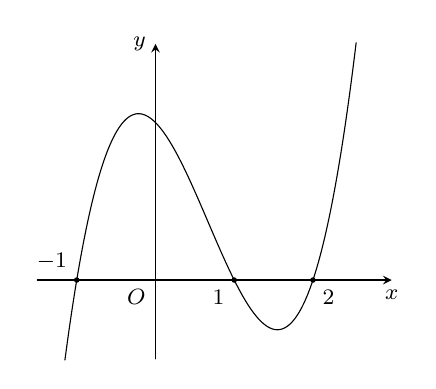
\begin{tikzpicture}[scale=1,font=\footnotesize,line join=round,line cap=round,>=stealth]
			 \draw[->] (-1.5,0)--(3,0) node[below] {$x$};
			\draw[->] (0,-1)--(0,3) node[left]  {$y$};
			\draw (0,0) node  [below left] {$O$};
			\fill (-1,0)  circle (1pt) node[above left] {$-1$}
				(1,0) circle (1pt) node[below left]  {$1$}
				(2,0) circle (1pt)  node[below right] {$2$};
			 \draw[smooth,samples=200] plot[domain=-1.15:2.55] (\x,{(\x)^3-2*(\x)^2-(\x)+2});
		\end{tikzpicture}
	\end{center}
	Kết luận nào sau đây là  đúng?
	\choice 
		{\True $f(3)<f(4)$} 
		{$f(-2)<f(-1)$} 
		{$f(3)>f(4)$} 
		{$f'(0)=0$} 
	\loigiai{ 
		 Trong khoảng $(2;+\infty)$ hàm số đồng biến, các giá trị $x$ bằng $3$; $4$ thuộc khoảng $(2;+\infty)$.\\
		Suy  ra $f(3)<f(4)$.
	 }
\end{ex}

% nguồn: Phan1_Lop_12_Dai_so_Chuong_1
\begin{ex}%[2D1H1-2]%[ma:8d08f7cb]
	Cho  hàm số $y=f(x)$ có bảng biến thiên sau:
	\begin{center}
		
\begin{tikzpicture}
			 \tkzTabInit[lgt=1.2,espcl=2.5,deltacl=0.6]
				{$x$ /1.0,$y'$ /0.6,$y$ /2} 
				 {$-\infty$,$-3$,$-2$,$-1$,$+\infty$}
			\tkzTabLine{,+,z,-,d,-,z,+,} 
			 \tkzTabVar{-/$-\infty$,+/ $-2$,-D+/$-\infty$/$+\infty$,-/$0$,+/$+\infty$}
		\end{tikzpicture}
	\end{center}
	Hàm số đã cho đồng biến trên khoảng nào dưới  đây?
	\choice 
		{\True  $(0;+\infty)$}
		{$(-\infty;-2)$} 
		{$(-2;+\infty)$} 
		 {$\left(-\dfrac{3}{2};+\infty\right)$}
	\loigiai{ 
		Hàm  số đã cho đồng biến trên khoảng $(0;+\infty)$.
	} 
\end{ex}


%%%%%%%%%%%%%%%% ĐÚNG/SAI %%%%%%%%%%%%%%%%

% nguồn: Phan1_Lop_12_Dai_so_Chuong_1
\begin{ex}%[2D1H1-2]%[ma:59c122fe]
	Cho hàm số $y=f(x)$ liên tục  trên $\mathbb{R}$ và có bảng biến thiên như sau
	\begin{center}
		
\begin{tikzpicture}
			 \tkzTabInit[nocadre=true,lgt=1.2,espcl=3,deltacl=0.5]
				{$x$/.7,$f'(x)$/.7,$f  (x)$/2}
				 {$-\infty$,$-1$,$1$,$+\infty$}
			 \tkzTabLine{,-,$0$,+,$0$,-,}
			\tkzTabVar{+/$142$,-/$8$,+/$38$,-/$14$} 
		\end{tikzpicture}
	\end{center}
	 \choiceTF
		 {\True Hàm số đã cho nghịch biến trên khoảng $\left(8;14\right)$}
		{\True Hàm số đạt giá trị nhỏ  nhất bằng $8$}
		{Hàm số đạt giá trị  lớn nhất bằng $38$}
		{Hàm số  đã cho đồng biến trên $(8;38)$}
	\loigiai{\begin{itemchoice}
		\itemch  {\bf Đúng}.\\
		Vì hàm số nghịch biến trên  $(-\infty;-1)$ và $(1;+\infty)$ do đó cũng nghịch biến trên $(8;14)$.
		\itemch  {\bf Đúng}.\\
		Dựa vào bảng biến thiên ta thấy giá trị nhỏ  nhất là $8$ tại $x=-1$.
		\itemch {\bf Sai}.\\ 
		Hàm số không  có giá trị lớn nhất.
		 \itemch {\bf Sai}.\\
		Hàm số đồng biến trên $(-1;1)$ do  đó không đồng biến trên $(8;38)$.
	\end{itemchoice}
 }
\end{ex}

% nguồn: Phan1_Lop_12_Dai_so_Chuong_1
\begin{ex}%[2D1H1-2]%[ma:3b4138fd]
	Cho hàm  số $y=f(x)=\dfrac{ax^2+bx+c}{mx+n}$ (với $a, m\neq 0$) có đồ thị là~đường cong như hình
	\begin{center}
		\resizebox{!}{5cm}{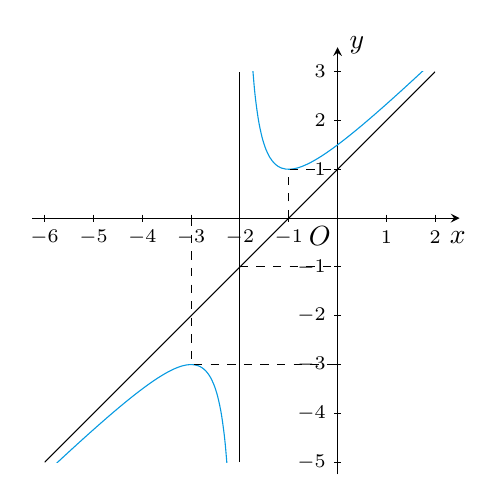
\begin{tikzpicture}[line cap=butt,line join=miter,>=stealth,xscale=0.62,yscale=0.62]
		 \tikzset{declare function={xmin=-6; xmax=2; Xkxd=-2;
			ymin=-5; ymax=3; 
			a=1; b=3; c=3; d=1;  et=2;
			akxd=1;  bkxd=1;
			f (\x)=(a*(\x)^2+b*\x+c)/(d*(\x)+et); 
			 h (\x)=akxd*\x+bkxd;
			 },
			 smooth,samples=50
		} 
		\draw[->]  (xmin-0.25,0)--(xmax+0.5,0)
			node[shift={(-95:7pt)},font=\normalsize]{$ x $}; 
		\draw[->]  (0,ymin-0.25)--(0,ymax+0.5)
			node[shift={(5:7pt)},font=\normalsize]{$ y $}; 
		\fill (0,0) node[shift={(225:9pt)},font=\normalsize]{$ O $}; 
		\foreach \x in  {-6,-5,-4,-3,-2,-1,1,2}{
			\draw (\x,2pt)--(\x,-2pt)  +(0,-9pt) node[font=\scriptsize,inner sep=1pt]{$\x$};
		 }
		\foreach  \y in {-5,-4,-3,-2,-1,1,2,3}{
			\draw (2pt,\y)--(-2pt,\y)  +(-3pt,0) node[font=\scriptsize,anchor=east,inner sep=1pt]{$\y$};
		} 
		\begin{scope}
			\clip (xmin,ymin) rectangle (xmax,ymax); 
			\draw (Xkxd,ymin)--(Xkxd,ymax); 
			\draw plot[domain=xmin:xmax]  (\x,{h (\x)});
			\draw[cyan!85!blue] plot[domain=xmin:{Xkxd-0.05}]  (\x,{f (\x)});
			 \draw[cyan!85!blue] plot[domain={Xkxd+0.05}:xmax] (\x,{f (\x)});
		\end{scope}
		\draw[dashed] (-3,0)--(-3,-3)--(0,-3) 
			(-1,0)--(-1,1)--(0,1) 
			(-2,-1)--(0,-1); 
	\end{tikzpicture}
		} 
	\end{center}
	 \choiceTF
		{\True Hàm số đồng  biến trên các khoảng $(-\infty;-3)$ và $(-1;+\infty)$}
		{\True $f(2024)  < f(2025)$}
		{Đồ thị  hàm số có tiệm cận đứng $x=-3$ và đường tiệm cận xiên $y=x+1$}
		{\True Đồ  thị hàm số đi qua điểm $A\left(2;\dfrac{13}{4}\right)$}
	 \loigiai{
		\begin{itemchoice}
			\itemch Nhìn đồ thị ta thấy mệnh  đề \textbf{đúng}.
			\itemch Do hàm số đồng biến trên khoảng  $(-1;+\infty)$, suy ra mệnh đề \textbf{đúng}.
			\itemch Nhìn đồ thị ta thấy đồ thị hàm số có tiệm cận đứng $x=-2$ và đường tiệm cận xiên đi qua  hai điểm $A\left(-1;0\right)$, $B\left(0;1\right)$ nên có phương trình $y=x+1$, suy ra mệnh đề \textbf{sai}.
			\itemch Ta thấy đồ thị hàm số có tiệm cận đứng $x=-2$ và đường tiệm cận xiên $y=x+1$. Dựa vào công thức thì đồ thị hàm số có tiệm cận đứng $x=-\dfrac{n}{m}$ và đường tiệm cận xiên $y=\dfrac{a}{m} x+\dfrac{b}{m}-\dfrac{an}{m^2}$. Từ đó suy  ra $\heva{&\dfrac{-n}{m}=-2 \\ &\dfrac{a}{m}=1 \\ &\dfrac{b}{m}-\dfrac{an}{m^2}=1}
			\Rightarrow \heva{&n=2m  \\ &a=m \\ &b=3m.}$\\
			 Do đó hàm số có dạng $y=f(x)=\dfrac{mx^2+3mx+c}{mx+2m}$.\\
			Đồ thị hàm số  đi qua điểm $M\left(-1;1\right)\Rightarrow 1=\dfrac{m-3m+c}{-m+2m} \Rightarrow c=3m$.\\
			Vậy hàm số có  dạng $y=f(x)=\dfrac{mx^2+3mx+3m}{mx+2m}=\dfrac{x^2+3x+3}{x+2}$.\\
			Ta  có $\dfrac{13}{4}=\dfrac{2^2+3\cdot2+3}{2+2}$ (đúng), nên đồ thị hàm số đi qua điểm $A\left(2;\dfrac{13}{4} \right)$, suy ra mệnh đề \textbf{đúng}.
		\end{itemchoice}
	} 
\end{ex}

% nguồn: Phan1_Lop_12_Dai_so_Chuong_1
\begin{ex}%[2D1H1-2]%[ma:4b56d586]
	Cho hàm số $y=f(x)$ liên tục trên các khoảng xác định  và có bảng biến thiên như hình vẽ sau:
	\begin{center}
		\resizebox{0.8\linewidth}{!}{
\begin{tikzpicture}
		 \tkzTabInit{$x$/1,$y'$/1,$y$/3}
			 {$-\infty$,$-2$,$0$,$2$,$+\infty$}
		 \tkzTabLine{,+,d,+,d,+,0,-,}
		\tkzTabVar{-/$2$,+D-/$+\infty$/$-\infty$,+D-/$1$/$-\infty$,+/$1$,-/$-3$} 
	\end{tikzpicture}
		 }
	\end{center}
	Xét tính đúng,  sai của các mệnh đề sau:
	 \choiceTF
		{\True Số đường tiệm cận đứng của đồ thị hàm số đã cho là~$2$} 
		{Đồ thị hàm số  $y=f(x)$ có hai đường tiệm cận ngang $y=2$; $y=3$}
		{\True Hàm số $y=f(x)$ nghịch biến trong khoảng $\left(1;+\infty \right)$} 
		{Hàm số $y=f(x)$ có hai điểm cực trị} 
	\loigiai{ 
		\begin{itemchoice}
			\itemch\textbf{Đúng.} 
			\begin{itemize}
				\item Ta  có $\heva{&\mathop{\lim y}\limits_{x\to-2^{+}}=-\infty \\ &\mathop{\lim y}\limits_{x\to-2^{-}}=+\infty}\Rightarrow x=-2$ là~tiệm cận đứng của đồ thị hàm số.\\
				\item ${\mathop{\lim y}\limits_{x\to 0^{+}}}=-\infty \Rightarrow x=0$ là~tiệm cận đứng của đồ thị hàm số. 
			\end{itemize}
			\itemch \textbf{Sai.} 
			\begin{itemize}
				\item${\mathop{\lim y}\limits_{x\to-\infty}}=2\Rightarrow$ Đồ thị hàm số có tiệm cận ngang $y=2$. 
				\item ${\mathop{\lim  y}\limits_{x\to+\infty}}=-3\Rightarrow$ Đồ thị hàm số có tiệm cận ngang $y=-3$.
			\end{itemize}
			\itemch \textbf{Đúng.} 
			Trong khoảng  $\left(1;+\infty \right)$, $y' < 0$
			 \itemch
			\textbf{Sai.}\\ 
			Từ bảng biến thiên ta thấy hàm số $y=f(x)$ đối dấu duy nhất một lần khi qua $x_0=2$.\\ $\Rightarrow$ Đồ thị hàm số $y=f(x)$ có duy nhất  duy nhất một điểm cực trị.
	\end{itemchoice}}
\end{ex}

% nguồn: Phan1_Lop_12_Dai_so_Chuong_1
\begin{ex}%[2D1H1-2]%[ma:e410a7ad]
	 Cho hàm số $y=f\left(x\right)$ có đồ thị như hình vẽ.
	\begin{center}
		\begin{tikzpicture}[scale=1,font=\footnotesize,line join=round,line cap=round,>=stealth]
			\draw[->] (-2,0)--(0,0) node[below  left]{$O$}--(3.5,0) node[above]{$x$};
			 \foreach \x in {1,2}
			 \draw[shift={(\x,0)}] (0pt,2pt)--(0pt,-2pt)
				node[below]  {$\x$};
			\draw[->] (0,-1)--(0,4)  node[right]{$y$};
			\foreach  \y in {1,2,3}
			 \draw[shift={(0,\y)}] (2pt,0pt) -- (-2pt,0pt)
				node[left]  {$\y$};
			\clip (-2,-1) rectangle  (4,4);
			 \draw[smooth,red,line width=1] plot[domain=-1:1.8] (\x,{2*(\x)^(3)-3*(\x)^(2)+3});
			 \draw[dashed] (1,0)--(1,2)--(0,2);
		\end{tikzpicture}
	\end{center}
	 \choiceTF
		{\True  Hàm số nghịch biến trên khoảng $\left(0;1\right)$}
		{\True Hàm số đạt cực trị các điểm $x=0$ và $x=1$} 
		{\True Hàm số đồng biến trên  các khoảng $\left(-\infty;0\right)$ và $\left(1;+\infty\right)$}
		{$f(0)<f(1)$} 
	\loigiai{Từ  đồ thị ta thấy
		\begin{itemchoice}
			\itemch Hàm số nghịch biến trên khoảng  $\left(0;1\right)$.
			\itemch Hàm số đạt cực trị các điểm $x=0$ và $x=1$. 
			\itemch Hàm số  đồng biến trên các khoảng $\left(-\infty;0\right)$ và $\left(1;+\infty\right)$.
			 \itemch Vì hàm số nghịch biến trên khoảng $\left(0;1\right)$, ta có $0<1\Rightarrow f(0)>f(1)$.
		\end{itemchoice}
	} 
\end{ex}

% nguồn: Phan1_Lop_12_Dai_so_Chuong_1
\begin{ex}%[2D1H1-2]%[ma:e27f050a]
	Cho hàm số $y=f(x)$  xác định trên $\mathbb{R}$ có bảng xét dấu đạo hàm như sau:
	\begin{center}
		
\begin{tikzpicture}\tkzTabInit[nocadre,lgt=1.5,espcl=2,deltacl=.5]
				{$x$/0.7,$f’(x)$/0.7}{$-\infty$,$0$,$1$,$2$,$+\infty$} 
			\tkzTabLine{,-,d,+,z,+,d,-,} 
		\end{tikzpicture}
	\end{center}
	 \choiceTF
		{\True Hàm số đồng biến trên  khoảng $(0;2)$}
		{\True Hàm số đồng  biến trên khoảng $(1;2)$}
		{Hàm số nghịch biến trên  khoảng $(-\infty;+\infty)$}
		{\True Hàm số nghịch biến trên các khoảng $(-\infty;0)$  và $(2;+\infty)$}
	 \loigiai{
		\begin{itemchoice}
			\itemch \textbf{Đúng}. Vì dựa vào bảng xét  dấu đạo hàm, hàm số đồng biến trên khoảng $(0;2)$.
			\itemch \textbf{Đúng}. Vì dựa vào  bảng xét dấu đạo hàm, hàm số đồng biến trên khoảng $(1;2)$.
			\itemch \textbf{Sai}. Vì dựa vào bảng xét dấu đạo  hàm, hàm số không nghịch biến trên khoảng $(-\infty;+\infty)$.
			\itemch \textbf{Đúng}. Vì dựa vào bảng xét dấu đạo  hàm, hàm số nghịch biến trên các khoảng $(-\infty;0)$ và $(2;+\infty)$.
		\end{itemchoice}
	 }
\end{ex}

% nguồn: Phan1_Lop_12_Dai_so_Chuong_1
\begin{ex}%[2D1V1-2]%[ma:3ebb5e0a]
	Cho hàm số $f(x)=\dfrac{ax+b}{cx+d}$ với $a,b,c,d\in \mathbb{R}$ có đồ thị hàm số $y=f'(x)$ nhận $x=-1$ làm tiệm cận đứng như hình vẽ. Biết rằng giá trị lớn nhất của hàm số $y=f(x)$ trên đoạn $[-3;-2]$  bằng $8$.
	\begin{center}
		\begin{tikzpicture}[scale=0.7,font=\footnotesize,line join=round,line cap=round,>=stealth]
			 \draw[->] (-5,0) -- (5,0) node[below] {$x$};
			\draw[->] (0,-1) --  (0,5) node[right] {$y$};
			\filldraw (0,0) node[below left=-0.05]  {$O$} circle (1.2pt);
			\draw[smooth,samples=100,domain=-5:-1.6]  plot (\x,{-3/(\x+1)});
			\draw[smooth,samples=100,domain=-0.4:5] plot (\x,{3/(\x+1)}); 
			\draw (0,3) node[left]{$3$} circle  (1.5pt)
				(-1,0) node[below]{$-1$}  circle (1.5pt);
			\draw (-1,-1)--(-1,5); 
		\end{tikzpicture}
	\end{center}
	\choiceTF 
		{\True $f'(0)=3$} 
		{Hàm số $y=f(x)$ nghịch biến trên khoảng $(-1;+\infty)$} 
		 {Giá trị của $f(-3)$ bằng $8$}
		{\True Giá trị của  $f(2)$ bằng $4$}
	\loigiai{ 
		\begin{itemchoice}
			 \itemch
			Theo hình vẽ, đồ thị $f'(x)$ qua  điểm $(0;3)$ nên $f'(0)=3$.
			 \itemch
			Do $f'(x)>0,\forall x\neq-1$ nên hàm số đã cho $f(x)$ đồng  biến trên các khoảng $(-\infty;-1)$ và $(-1;+\infty)$.
			\itemch Do $f'(x)>0,\forall x\neq-1\Rightarrow\max\limits_{[-3;-2]} f(x)=f(-2)=8$ suy ra $f(-3) \neq  8$.
			 \itemch
			Ta có  $f'(x)=\dfrac{ad-bc}{(cx+d)^2}$.\\
			Đồ  thị hàm số đi qua điểm $(0;3)$ nên $f'(0)=3 \Leftrightarrow \dfrac{ad-bc}{d^2}=3$.\\
			Mặt khác, đồ thị hàm số $y=f'(x)$ có tiệm  cận đứng $x=-1$ nên $-c+d=0$.\\
			Vì $f'(x)>0,\forall x\neq1$ nên $\max\limits_{[-3;-2]}  f(x)=f(-2)=8\Leftrightarrow\dfrac{-2a+b}{-2c+d}=8$.\\
			Vậy ta có hệ phương trình $\left\{\begin{aligned}
			 &ad-bc=3d^2\\
			 &-c+d=0\\
			&b-2a=8(d-2c) 
		\end{aligned}\Leftrightarrow\left\{\begin{aligned}
		&c=d\\ 
		&a-b=3d\\ 
		 &b-2a=-8d
	\end{aligned}\Leftrightarrow\left\{\begin{aligned}
	&a=5d\\ 
	 &b=2d\\
	 &c=d.
	\end{aligned}\right.\right.\right.$\\
	Từ đó suy ra $f(x)=\dfrac{5dx+2d}{dx+d}=\dfrac{5x+2}{x+1} \Rightarrow  f(2)=4$.
	\end{itemchoice}
	} 
	\end{ex}

% nguồn: Phan1_Lop_12_Dai_so_Chuong_1
\begin{ex}%[2D1V1-2]%[ma:a1e39981]
		Cho hàm số $y = f(x)$ xác định trên $\mathbb{R}$, có đồ thị $f'(x)$ như hình vẽ bên dưới đây. 
		\begin{center}
			\begin{tikzpicture}[line join=round,line cap=round,>=stealth,scale=0.5]
				\tikzset{ethicknode/.style={scale=0.9}} 
				\draw[->] (-7.1,0)--(9.1,0) node[below  left] {$x$};
				 \draw[->] (0,-2.1)--(0,5.1) node[below left] {$y$};
				\draw  (0,0) node [above left] {$O$};
				\foreach \x/\nx in {-6/-6,-2/-2,1/1,8/8} 
				\draw[thin] (\x,1pt)--(\x,-1pt)  node [below] {$\nx$};
				\begin{scope}
					\clip (-7,-2)  rectangle (9,7);
					\draw[samples=100,domain=-7:9,smooth,variable=\x] 
						 plot (\x,{-1/236*((\x)^4-(\x)^3-52*(\x)^2-44*(\x)+96)});
				\end{scope}
			\end{tikzpicture}
		\end{center}
		Xét tính đúng sai  của các mệnh đề sau:
	\choiceTF 
			{Hàm số $y =  f(x)$ có ba điểm cực trị}
			{\True Hàm số  $y = f(x)$ đồng biến trên khoảng $(1; 8)$}
			{Hàm  số $y = f(x)$ đạt cực đại tại $x = 1$}
			{\True  $\min\limits_{x \in (-\infty; -2)} f(x) = f(-6)$}
	 \loigiai{
		\begin{itemchoice}
			\itemch 
			 Ta có $f'(x) = 0 \Rightarrow
			\hoac{& x = -6 \\& x  = -2 \\& x = 1 \\& x = 8 }$.\\
			Bảng xét  dấu của $f'(x)$
			\begin{center}
			
\begin{tikzpicture}
				 \tkzTabInit[deltacl=0.5,espcl=2.5,lgt=2,nocadre]
					 {$x$/1,$f'(x)$/1}
					 {$-\infty$,$-6$,$-2$,$1$,$8$,$+\infty$}
				 \tkzTabLine{,-,0,+,0,-,0,+,0,-,}
			\end{tikzpicture}
			\end{center}
			Hàm số $y = f(x)$ có bốn điểm cực trị tại $x = -6$, $x  = -2$, $x = 1$, và $x = 8$.
			\itemch 
			Hàm số  đồng biến trên khoảng $(1; 8)$.
			 \itemch
			Hàm  số đạt cực tiểu tại $x = 1$.
			\itemch 
			Trên $(-\infty; -2)$, hàm số có giá trị  nhỏ nhất tại $f(-6)$.
		\end{itemchoice}
	 }
\end{ex}


%%%%%%%%%%%%%%%% TRẢ LỜI NGẮN %%%%%%%%%%%%%%%%

% nguồn: Phan2_Lop_12_Dai_so_Chuong_1
\begin{bt}%[2D1N1-2]%[ma:6efe57e2]
	Cho đồ thị hàm số có  đồ thị như hình vẽ bên. Hàm số $y=f(x)$ nghịch biến trên khoảng $\left(a;b\right)$. Tính $a+2b$.
	 \shortans{4}
	\begin{center}
		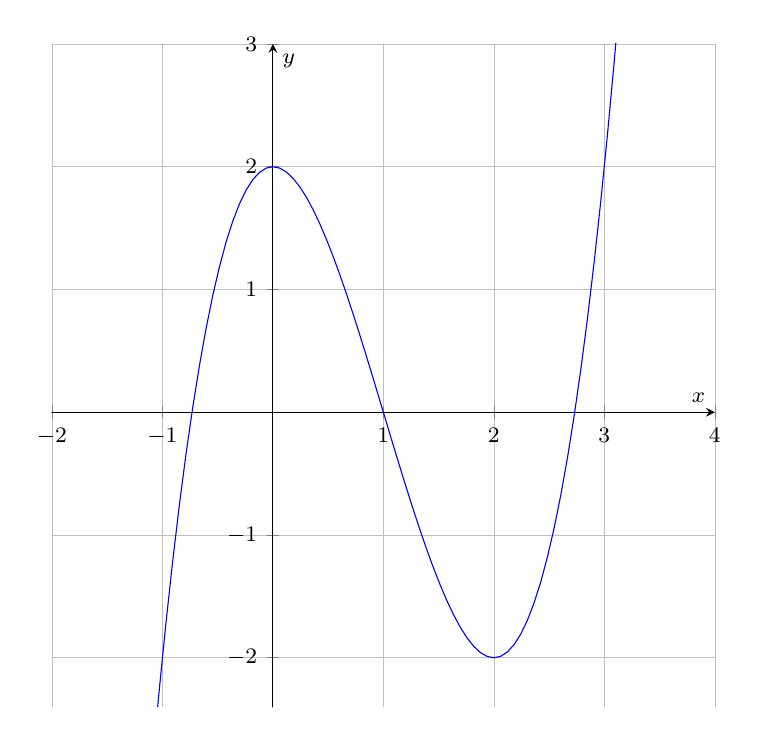
\begin{tikzpicture}[scale=1,font=\footnotesize,line join=round,line cap=round,>=stealth]
			\begin{axis}[
					axis lines =  middle,
					 xlabel = \(x\),
					 ylabel = \(y\),
					xmin =  -2,xmax = 4,
					ymin =  -2.4,ymax = 3,
					 grid = both,
					grid style = {line width=.1pt,draw,gray!10}, 
					major grid style =  {line width=.2pt,draw,gray!50},
					 width = 10cm,
					height = 10cm, 
					samples = 100, 
					domain = -2:4,] 
				\addplot [blue]  {x^3 - 3*x^2 + 2};
			\end{axis}
		\end{tikzpicture}
	\end{center}
	\loigiai{ 
		Dựa vào đồ thị hàm số ta  thấy hàm số $y=f(x)$ nghịch biến trên $\left(0;2\right)$.\\
		Suy  ra $a=0$, $b=2$.\\
	 Vậy $a+2b=4$.}
\end{bt}

% nguồn: Phan2_Lop_12_Dai_so_Chuong_1
\begin{bt}%[2D1H1-2]%[ma:296d2b8f]
	 \immini{
	Cho đồ thị hàm số $y=f(x)$ có đồ thị như hình vẽ bên. Hàm số $y=f(x)$ nghịch biến trên khoảng $(a;b)$. Tính giá trị lớn nhất của  $b-a$.
	\shortans{2} 
	 }{
	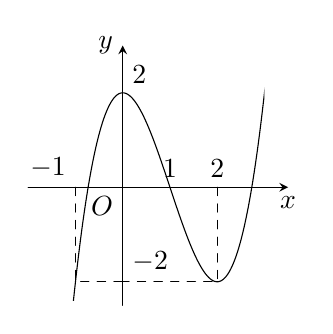
\begin{tikzpicture}[>=stealth,scale=0.6,line join=round,line cap=round]
		 \def\a{1} \def\b{-3} \def\c{0} \def\d{2}
		\def\xmin{-2} \def\xmax{3.5} \def\ymin{-2.5} \def\ymax{3} 
		\draw[->]  (\xmin,0)--(\xmax,0) node [below]{$x$};
		\draw[->] (0,\ymin)--(0,\ymax) node [left]{$y$}; 
		 \node at (0,0) [below left]{$O$};
		 \clip (\xmin+0.1,\ymin+0.1) rectangle (\xmax-0.5,\ymax-0.1);
		\draw[smooth,samples=300] plot  (\x,{\a*(\x)^3+\b*(\x)^2+\c*(\x)+\d});
		\draw[dashed](-1,0) node[above left]{$-1$}--(-1,-2)--(0,-2)  node[above right]{$-2$};
		\draw[dashed](2,0) node[above]{$2$}--(2,-2)--(0,-2); 
		\draw (1,0) node[above]{$1$};  \draw (0,2) node[above right]{$2$};
	\end{tikzpicture}
	 }
	 \loigiai{
		Dựa vào đồ thị hàm số ta thấy hàm số $y=f(x)$ nghịch biến trên  $(0;2)$.\\
		Suy ra $(a;b)\subset  (0; 2)$.\\
		Do đó $b-a$ lớn nhất khi $a=0$,  $b=2$.\\
		Vậy giá trị  lớn nhất của $b-a=2$.
	} 
\end{bt}

% nguồn: Phan2_Lop_12_Dai_so_Chuong_1
\begin{bt}%[2D1V1-2]%[ma:0444bc19]
	\immini{ 
	Đạo hàm $f'(x)$ của hàm số $f(x)$ là một hàm  số bậc hai và hàm số $y=f'(x)$ có đồ thị bên. Biết rằng hàm số $f(x)$ có giá trị cực đại là $2$ và giá trị cực tiểu là $-2$. Tìm giá trị của $f(2)$.
	 \shortans{18}}
	{\begin{tikzpicture}[line join=round,line cap = round,>=stealth,xscale=1.2,yscale=0.7,font=\footnotesize]
		\foreach  \x/\y/\z/\g in
			 {0/0/O/-55,-2/0/-2/-145}
		 \draw (\x,\y) circle (1pt) coordinate (\z)
			 ($(\z)+(\g:4.5mm)$) node{$\z$};
		\draw[->] (-3.1,0)--(2,0) node[below]{$x$}; 
		\draw[->] (0,-3)--(0,2.3) node[above]{$y$}; 
		\draw[smooth,samples=100,domain=-2.3:0.3] plot  (\x,{3*(\x)^2 +6*\x});
		\draw  (-1.3,2) node{$y=f'(x)$};
	\end{tikzpicture}
	 }
	\loigiai{ 
		Dựa vào đồ thị, ta thấy $f'(x)$ là hàm  số bậc hai có hai nghiệm là $0$ và $-2$\\ nên $f'(x)=ax(x+2)$ (với $a$ là số thực).\\
		Từ đó $\displaystyle f(x)=\int f'(x)\mathrm{\, d}x=a\left(\dfrac{x^3}{3}+x^2\right)+C$ ( với $C$ là hằng số).\\ 
		Từ đồ thị của $f'(x)$, ta  suy ra bảng biến thiên
		\begin{center}
			
\begin{tikzpicture}
				\tkzTabInit[nocadre=false,lgt=1.2,espcl=2.5,deltacl=0.7] 
					{$x$ /.6,$f'(x)$ /.6,$f (x)$ /2} 
					{$-\infty$,$-2$,$0$,$+\infty$} 
				\tkzTabLine{,+,$0$,-,$0$,+,} 
				\tkzTabVar{-/$-\infty$,+/$f (-2)$,-/$f  (0)$,+/$+\infty$}
			\end{tikzpicture}
		\end{center}
		Theo đề bài,  ta có $\heva{&f(-2)=2\\&f(0)=-2}\Rightarrow \heva{&C=-2\\& a\left(-\dfrac{8}{3}+4\right)-2=2}\Rightarrow\heva{&C=-2\\&a=3.}$\\
		Vậy $f(x)=x^3+3x^2-2$ và  $f(2)=18$.
	 }
\end{bt}
